\documentclass[a4paper,12pt]{article}

%\begin{figure}[htp]
%    \centering
%    \includegraphics[width=0.75\textwidth]{}
%\end{figure}

%%%%%%%%%%%%%%%%%%%%
%%%%  PREAMBLE  %%%%
%%%%%%%%%%%%%%%%%%%%
\usepackage{float}
\usepackage[T1]{fontenc}
\usepackage[utf8]{inputenc}

\usepackage[english,italian]{babel}
\usepackage{graphicx}     % Per includere immagini
\usepackage{subcaption}   % Per utilizzare subfigure
\usepackage{hyperref}
\usepackage{indentfirst}

\hypersetup{hidelinks}

\usepackage[margin=2.5cm]{geometry}
\usepackage{minipage-marginpar}
\usepackage{fancyhdr}
\usepackage[bottom]{footmisc}
\usepackage{lastpage}

\usepackage{enumitem}
\usepackage{tabularx}

\usepackage{graphicx}

\setlength{\parindent}{0em}
\setlength{\parskip}{1em}

\fancyhead[L]{\leftmark}
\fancyhead[R]{\shortstack[r]{Versione documento: 0.01 \\ Gruppo: G24}}

\fancyfoot[C]{}
\fancyfoot[R]{\thepage/\pageref{LastPage}}

\renewcommand{\headrulewidth}{2pt}
\renewcommand{\headruleskip}{3pt}
\setlength{\headheight}{30pt}

\renewcommand{\footrulewidth}{2pt}

\setlist[itemize]{itemsep=0.25em,topsep=0pt}
\setlist[enumerate]{itemsep=0.25em,topsep=0pt,align=left}

%%%%%%%%%%%%%%%%%%%%
%%%%  DOCUMENT  %%%%
%%%%%%%%%%%%%%%%%%%%

\title{}
\author{Gruppo G24}

\begin{document}

\pagestyle{empty}

\begin{center}

    \vspace{2 cm}

    \begin{tabular*}{\textwidth}{ c @{\extracolsep{\fill}} c }
        
\includegraphics[width=0.3\textwidth]{marchio_unitrento.pdf} & \shortstack{\Large{Dipartimento di Ingegneria} \\ \Large{e Scienza dell'Informazione}}
    \end{tabular*}

    \vspace{5 cm} 
  
    \Huge \textbf{Ingegneria del software\\}
  
    \vspace{1.5 cm} 
    \Large\textsc{Documento dei requisiti\\} 
    \vspace{3 cm} 
    \Huge\textsc{Mountain Wonders\\}
    \Large{Gruppo G24}
  
    \vspace{2 cm} 
  
    \Large{Anno accademico 2023/2024}
\end{center}

\newpage
\tableofcontents

\pagestyle{fancy}
\newpage
\section{Scopo del documento}

Il presente documento riporta la specifica dei requisiti di sistema del progetto MountainWonders. Lo scopo di questo documento è quello di mostrare le specifiche dei requisiti funzionali e non funzionali tramite l'utilizzo di diagrammi UML (Unified Modeling Language), diagrammi degli use-case, tabelle, context diagram e component diagram.\\
All'interno del documento precedentemente consegnato, sono stati specificati i requisiti funzionali e non funzionali in linguaggio naturale, mentre ora verranno espressi utilizzando un linguaggio più formale e strutturato.
    
\newpage

\section{Requisiti funzionali}

Vengono elencati di seguito i requisiti funzionali(RF) dell'applicazione, tramite l'utilizzo degli Use Case Diagram.

\subsection*{RF5 Account anonimo}

\subsubsection*{RF1 Registrazione}
\begin{figure}[H]
   \centering
    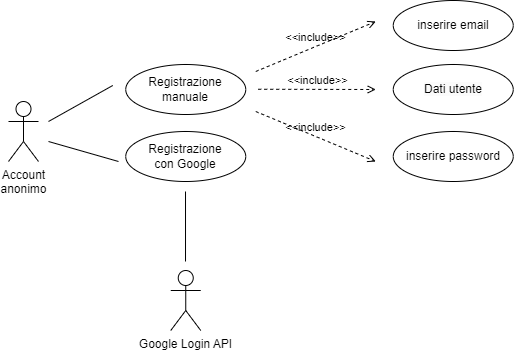
\includegraphics[width=0.8\textwidth]{img-D2/registrazione_anonimo.png}
    \caption{USE-CASE Registrazione}
\end{figure}


\subsubsection*{RF2 Login}
\begin{figure}[H]
   \centering
   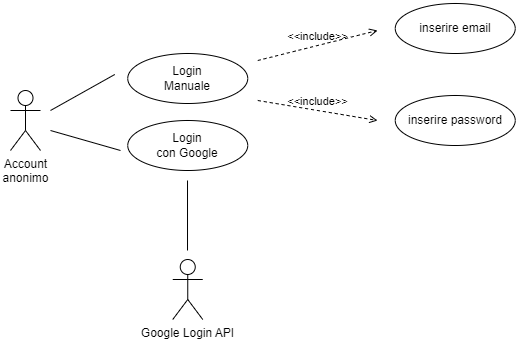
\includegraphics[width=0.8\textwidth]{img-D2/login_anonimo.png}
    \caption{USE-CASE Login}
\end{figure}

\subsubsection*{RF8 Ricerca}
\begin{figure}[H]
   \centering
   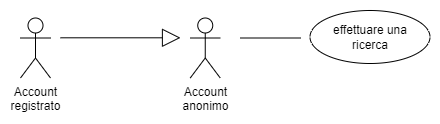
\includegraphics[width=0.7\textwidth]{img-D2/ricerca.png}
    \caption{USE-CASE Ricerca}
\end{figure}

\subsubsection*{RF7.1 Visualizza recensioni, RF9 Visualizzare montagne-rifugi}
\begin{figure}[H]
   \centering
   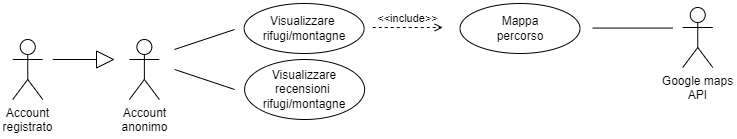
\includegraphics[width=1.0\textwidth]{img-D2/visualizzare_montagne.png}
    \caption{USE-CASE Visualizza Montagne-Rifugi-Recensioni}
\end{figure}


\subsubsection*{RF11 Supporto}
\begin{figure}[H]
   \centering
   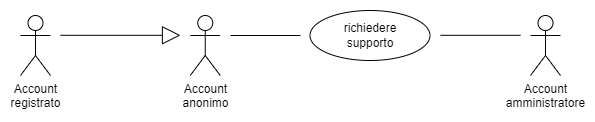
\includegraphics[width=1\textwidth]{img-D2/richiesta_supporto.png}
    \caption{USE-CASE Richiesta supporto}
\end{figure}

\subsubsection*{RF12 Cambio lingua}
\begin{figure}[H]
   \centering
   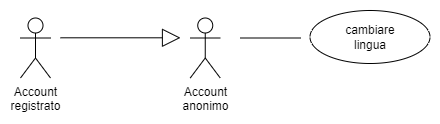
\includegraphics[width=0.8\textwidth]{img-D2/cambio_lingua.png}
    \caption{USE-CASE Cambio lingua}
\end{figure}

\subsubsection*{RF13 Meteo sulla Montagna}
\begin{figure}[H]
   \centering
   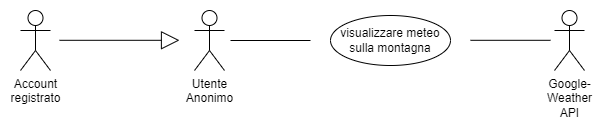
\includegraphics[width=1\textwidth]{img-D2/meteo.png}
    \caption{USE-CASE Meteo montagna}
\end{figure}


\subsection*{RF3 Account Amministratore}
\subsubsection*{RF2 Login}
\begin{figure}[H]
   \centering
   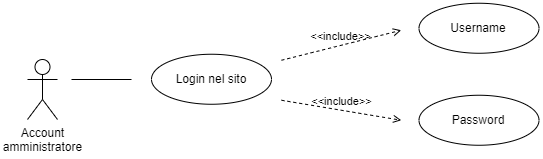
\includegraphics[width=0.6\textwidth]{img-D2/login_amministratore.png}
    \caption{USE-CASE Login}
\end{figure}

\subsubsection{RF3.1 Eliminare utenti registrati}

\subsubsection{RF3.2 Eliminare recensioni}

\subsubsection{RF3.3 Modificare/Eliminare montagna o rifugio}

\subsubsection{RF3.4 Rispondere alle richieste di supporto}





\subsection*{RF4 Account registrato}

Di seguito vengono descritte le funzioni dell'account registrato.

\subsubsection*{RF7 Recensioni}
\begin{figure}[H]
   \centering
   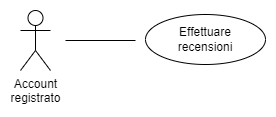
\includegraphics[width=0.5\textwidth]{img-D2/recensioni_registrato.png}
    \caption{USE-CASE Recensioni}
\end{figure}
 
\subsection*{RF6 Profilo utente}


\subsection*{RF10 Aggiungere rifugio o luogo di spicco}



\subsection*{RF9 Visualizzazione montagne}






\newpage
\subsection*{Tabella riassuntiva}

Di seguito è presente una tabella riassuntiva che associa ad ogni obiettivo, precedentmente descritto, i requisiti funzionali che permettono di raggiungerlo.

\begin{center}
    

\begin{tabular}{|l|l|}
\hline
Obiettivi     &Requisiti funzionale          \\
\hline
O1            & RF9, RF5\\ \hline 
O2            & RF1, RF2, RF4, RF7\\ \hline 
O3            & RF8, RF5\\ \hline 
O4            & RF3, RF11\\\hline
O5            & RF10\\\hline 
\end{tabular}
\newpage
\end{center}

\section{Requisiti non funzionali}

Vengono di seguito elencati e descritti i requisiti non funzionali del progetto. Ciascun requisito diversamente dai requisiti funzionali è legato alle performance.

\subsection*{RNF1 Sicurezza}



\subsection*{RNF2 Performance}



\subsection*{RNF3 Compatibilità}



\subsection*{RNF4 Affidabilità e disponibilità}



\subsection*{RNF5 Usabilità}



\subsection*{RNF6 Norme recensioni}


\subsection*{RNF7 Gestione delle immagini}



\subsection*{RNF8 Privacy}



\subsection*{RNF9 Aggiornamenti} 

 


\newpage
\section{Front-end}
Verranno mostrate di seguito le interfacce delle pagine web con relative descrizioni.
\subsection*{FE1 Homepage}
\begin{figure}[ht]
   \centering
    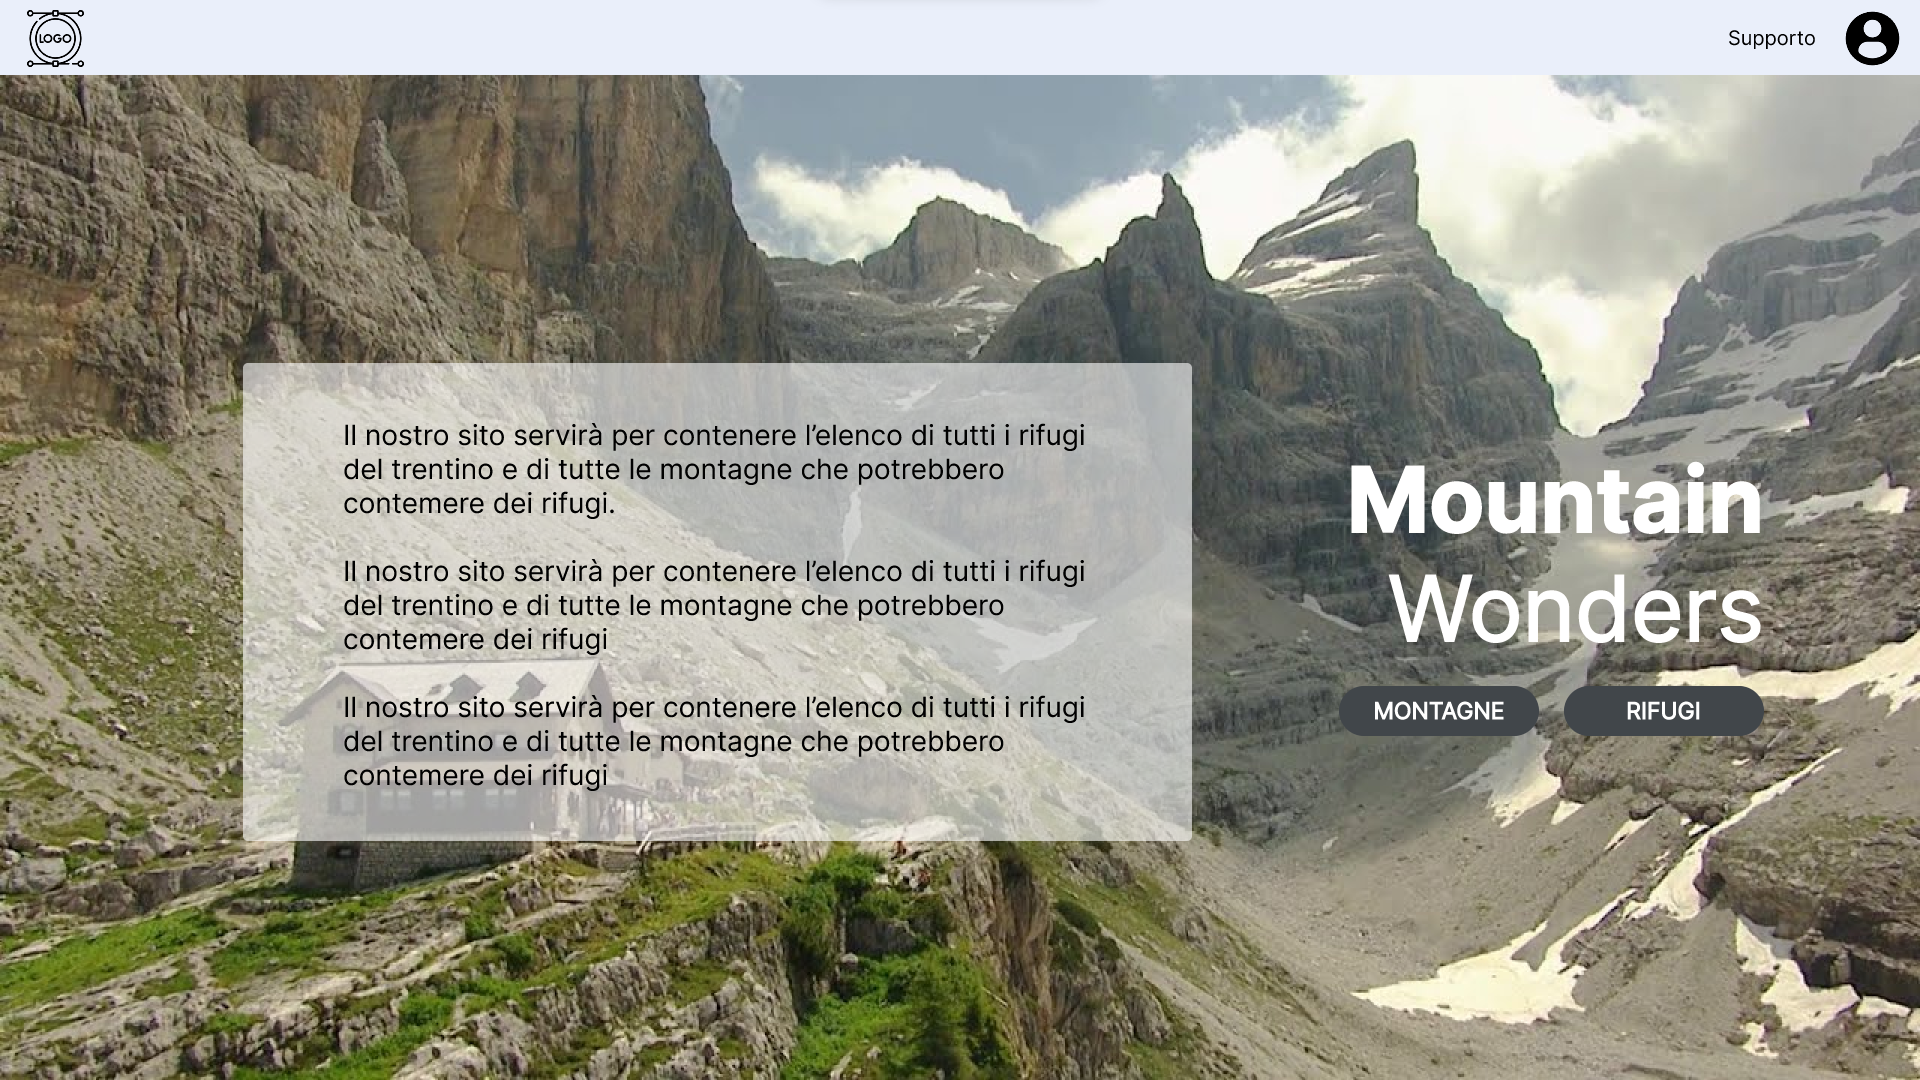
\includegraphics[width=0.6\textwidth]{img/Homepage.png}
    \caption{Homepage}
\end{figure}
Questa sarà la web page principale, da cui sarà possibile recarsi nelle seguenti pagine:
\begin{itemize}
    \item Profilo (RF6, nella barra di navigazione in alto a destra)
    \item Pagina delle montagne (RF9) (sotto il nome del sito)
    \item Pagina rifugi (RF9) (sotto il nome del sito)
\end{itemize}


\subsection*{FE2 Sign-up page}
\begin{figure}[H]
  \begin{subfigure}{0.49\textwidth}
    \centering
    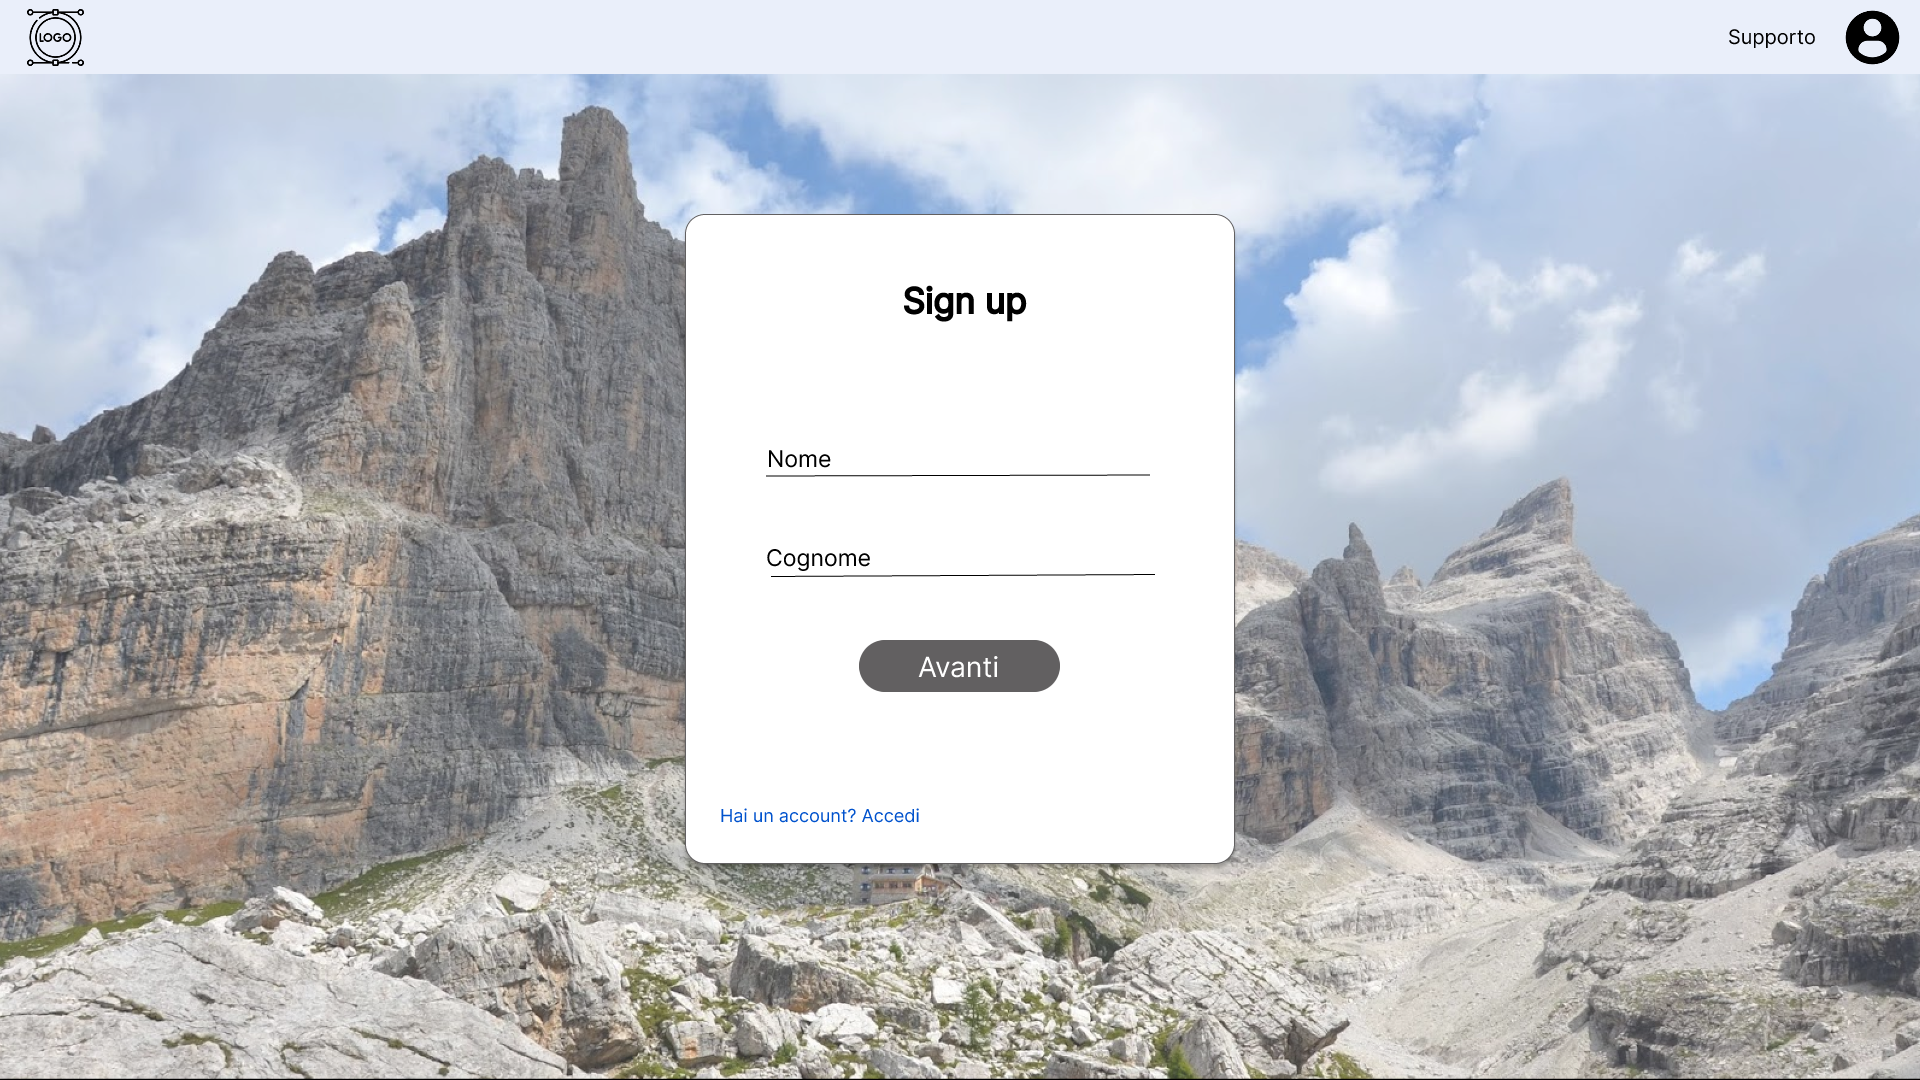
\includegraphics[width=\textwidth]{img/Sign-up 1.png} 
    \caption{Sign-up 1 pagina}
  \end{subfigure}
  \hfill % Spazio vuoto orizzontale tra le due immagini
  \begin{subfigure}{0.49\textwidth}
    \centering
    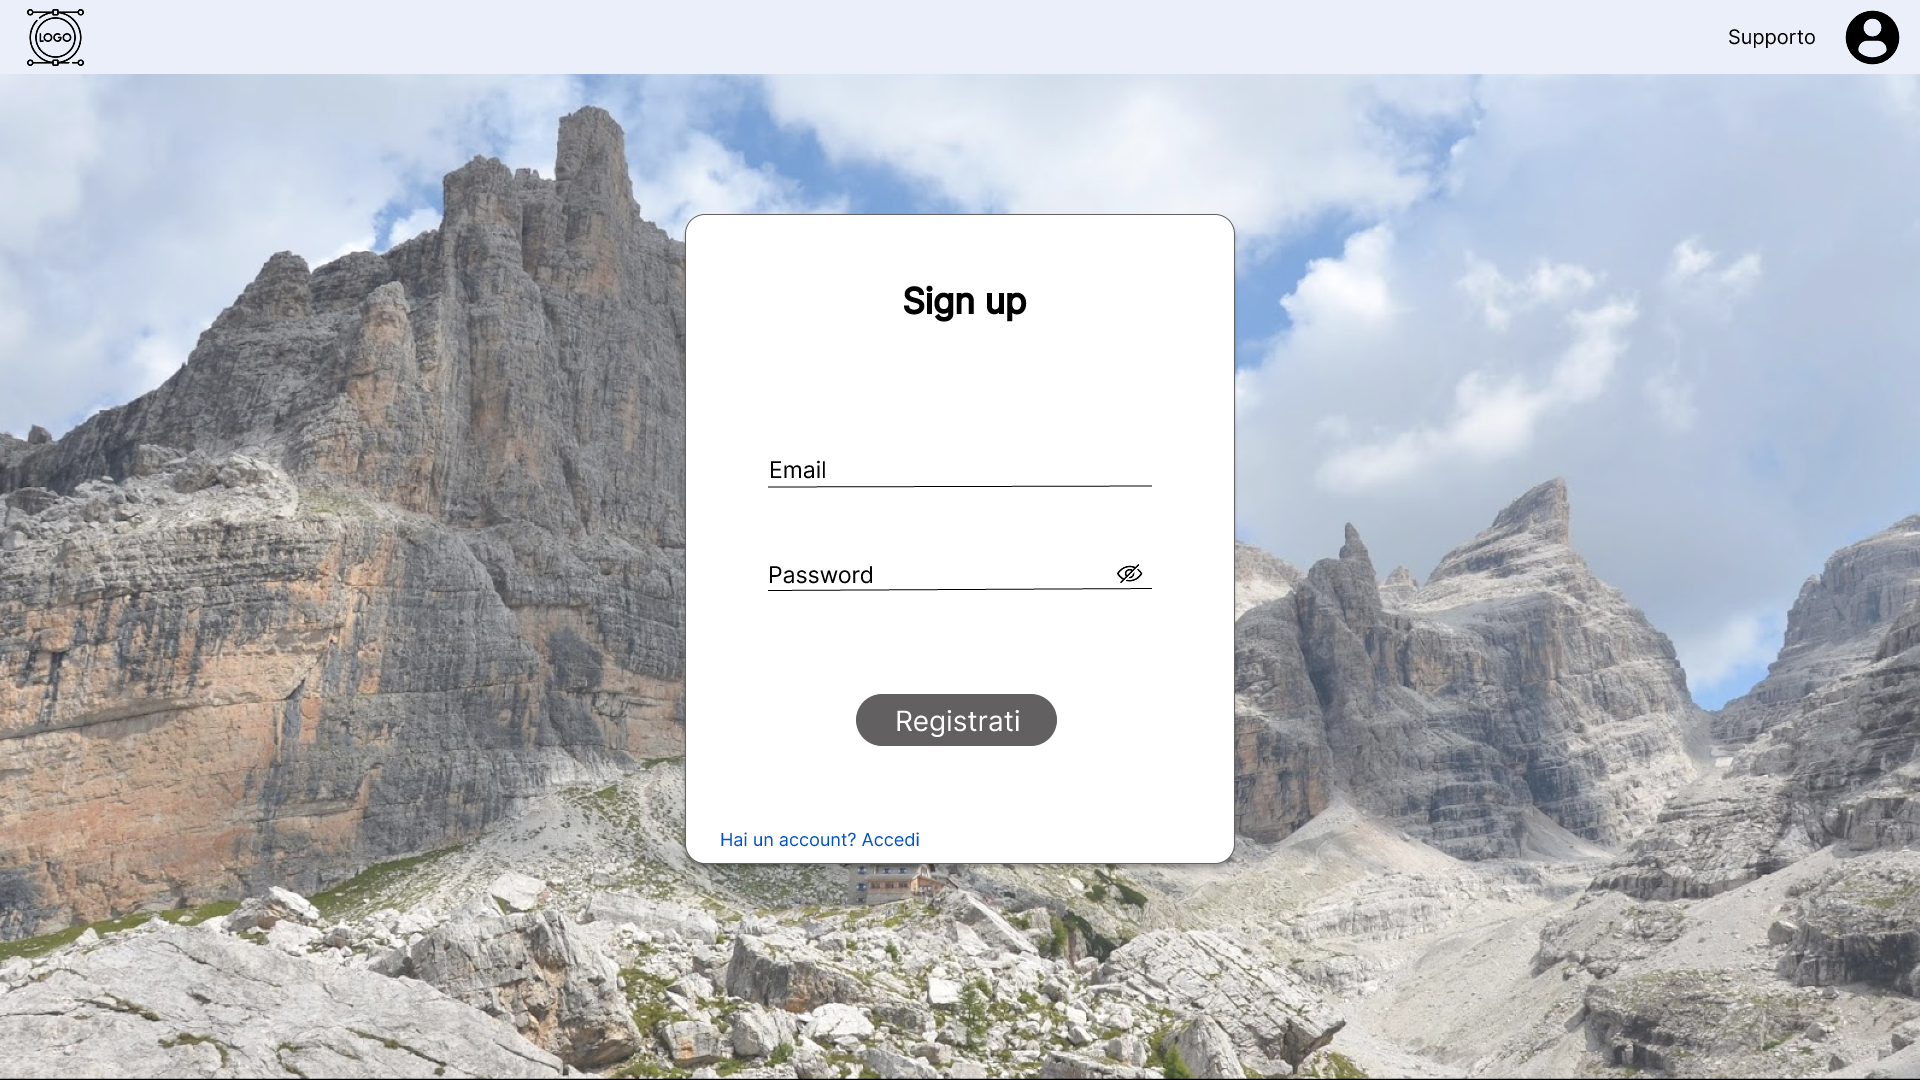
\includegraphics[width=\textwidth]{img/Sign-up 2.png} 
    \caption{Sign-up 2 pagina}
  \end{subfigure}
  \caption{Pagine di Sign-up (RF1)}
\end{figure}
All'interno di queste sezioni dedicate, sarà possibile compiere il processo di registrazione (RF1) per l'ingresso di nuovi utenti nel sito web. Nel primo passo di questo processo, verrà chiesto di fornire alcune informazioni fondamentali per la creazione dell'account personale, oppure sarà possibile registrarsi tramite il proprio account Google.

Nella prima sezione del modulo di registrazione, ci sarà la possibilità di inserire il nome e cognome. Questo passo iniziale è essenziale per garantire che l'account sia personalizzato e riconoscibile. Successivamente, si potrà procedere al passo successivo del processo, dove si avrà l'opzione di fornire ulteriori dettagli relativi al proprio account.

Nel secondo form, avrai la possibilità di inserire informazioni quali l'indirizzo email, che si intende associare al proprio account, e la password che si desidera utilizzare per l'accesso. L'email svolgerà un ruolo cruciale come mezzo di comunicazione e recupero dell'account, mentre la password garantirà la sicurezza dei tuoi dati personali (RNF1).


\subsection*{FE3 Log-in page}
\begin{figure}[H]
   \centering
    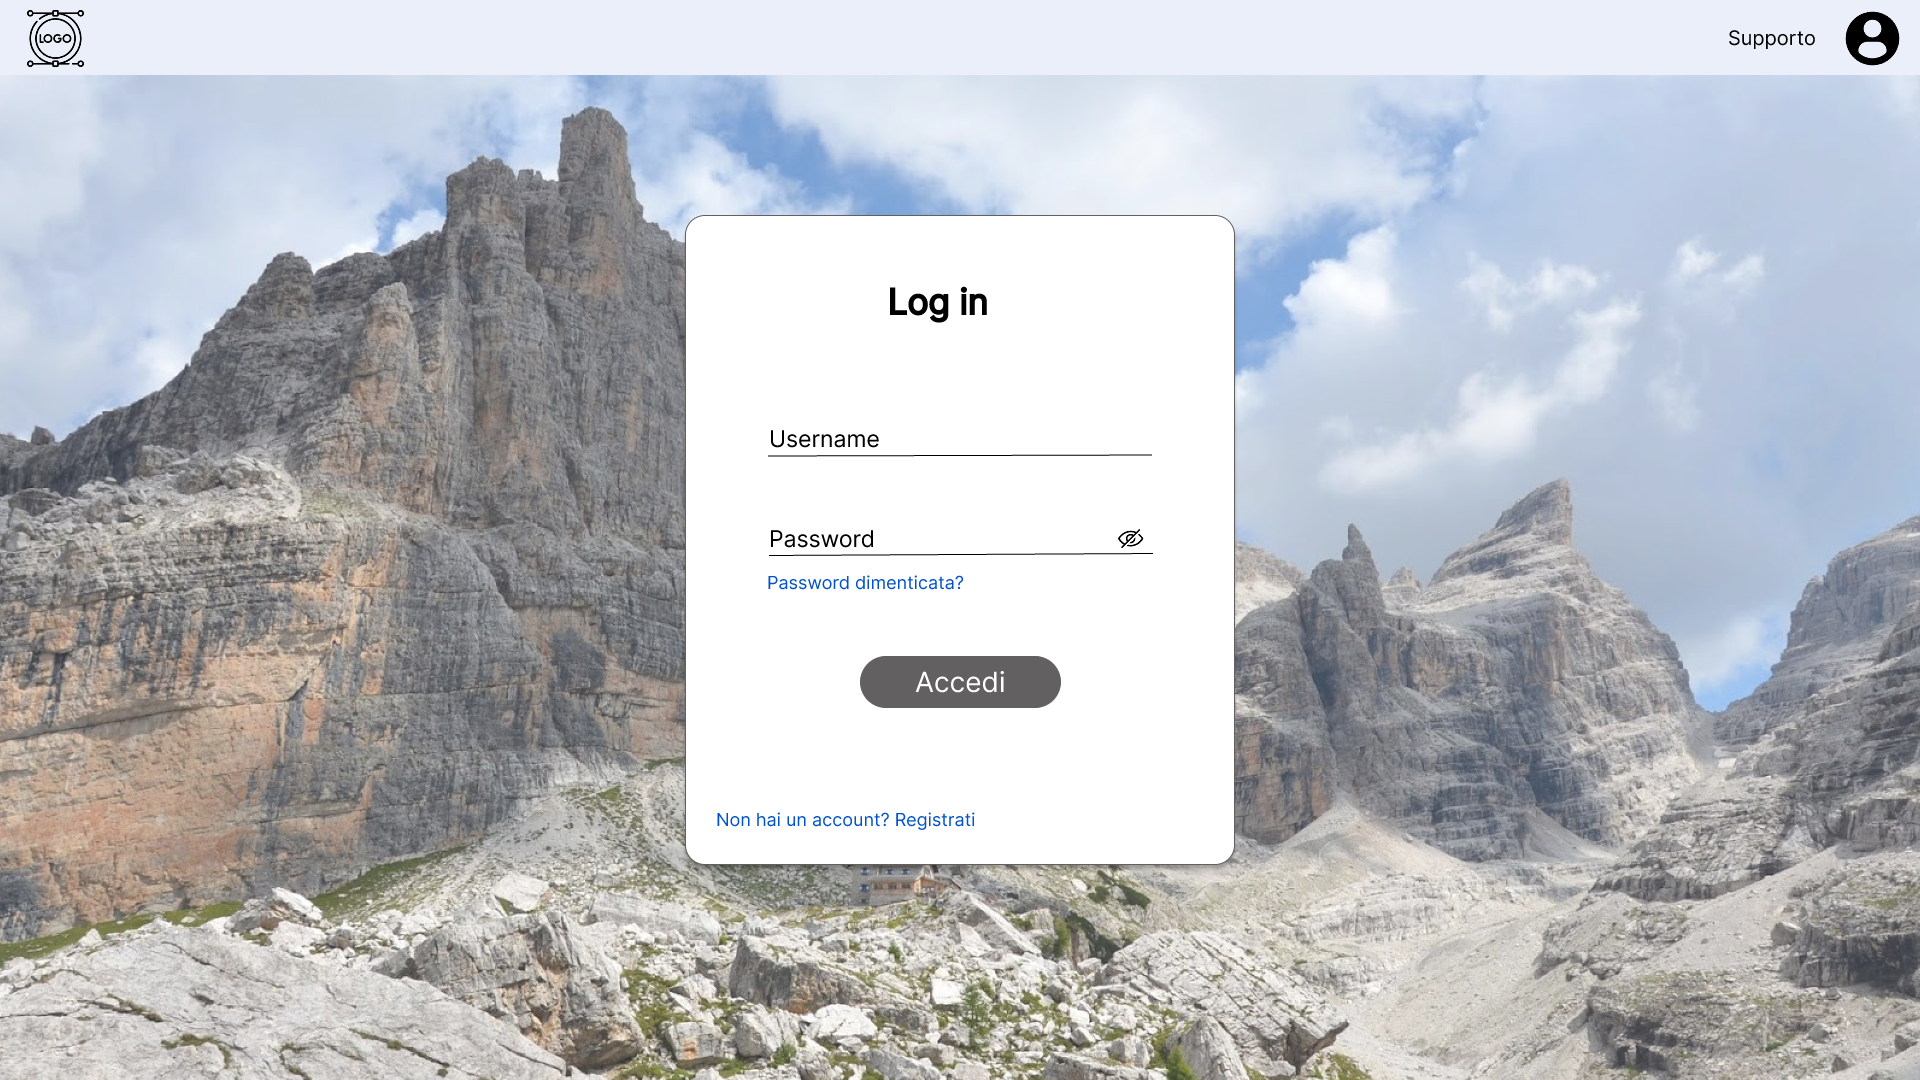
\includegraphics[width=0.6\textwidth]{img/Log-in.png}
    \caption{Pagina di log-in (RF2)}
\end{figure}
Questa pagina permetterà all'utente registrato di effettuare il login (RF2) tramite la propria email e la password oppure tramite il proprio account Google. Una volta inseriti basterà cliccare "Accedi" per effettuare il login. Nel caso in cui l'untente non dovesse ricordarsi la password potrà, cliccando il testo: "Password dimenticata?", richiedere una nuova password che gli sarà inviata via email all'inidirizzo fornito durante la registrazione.


\subsection*{FE4 Pagina montagne}
\begin{figure}[H]
   \centering
    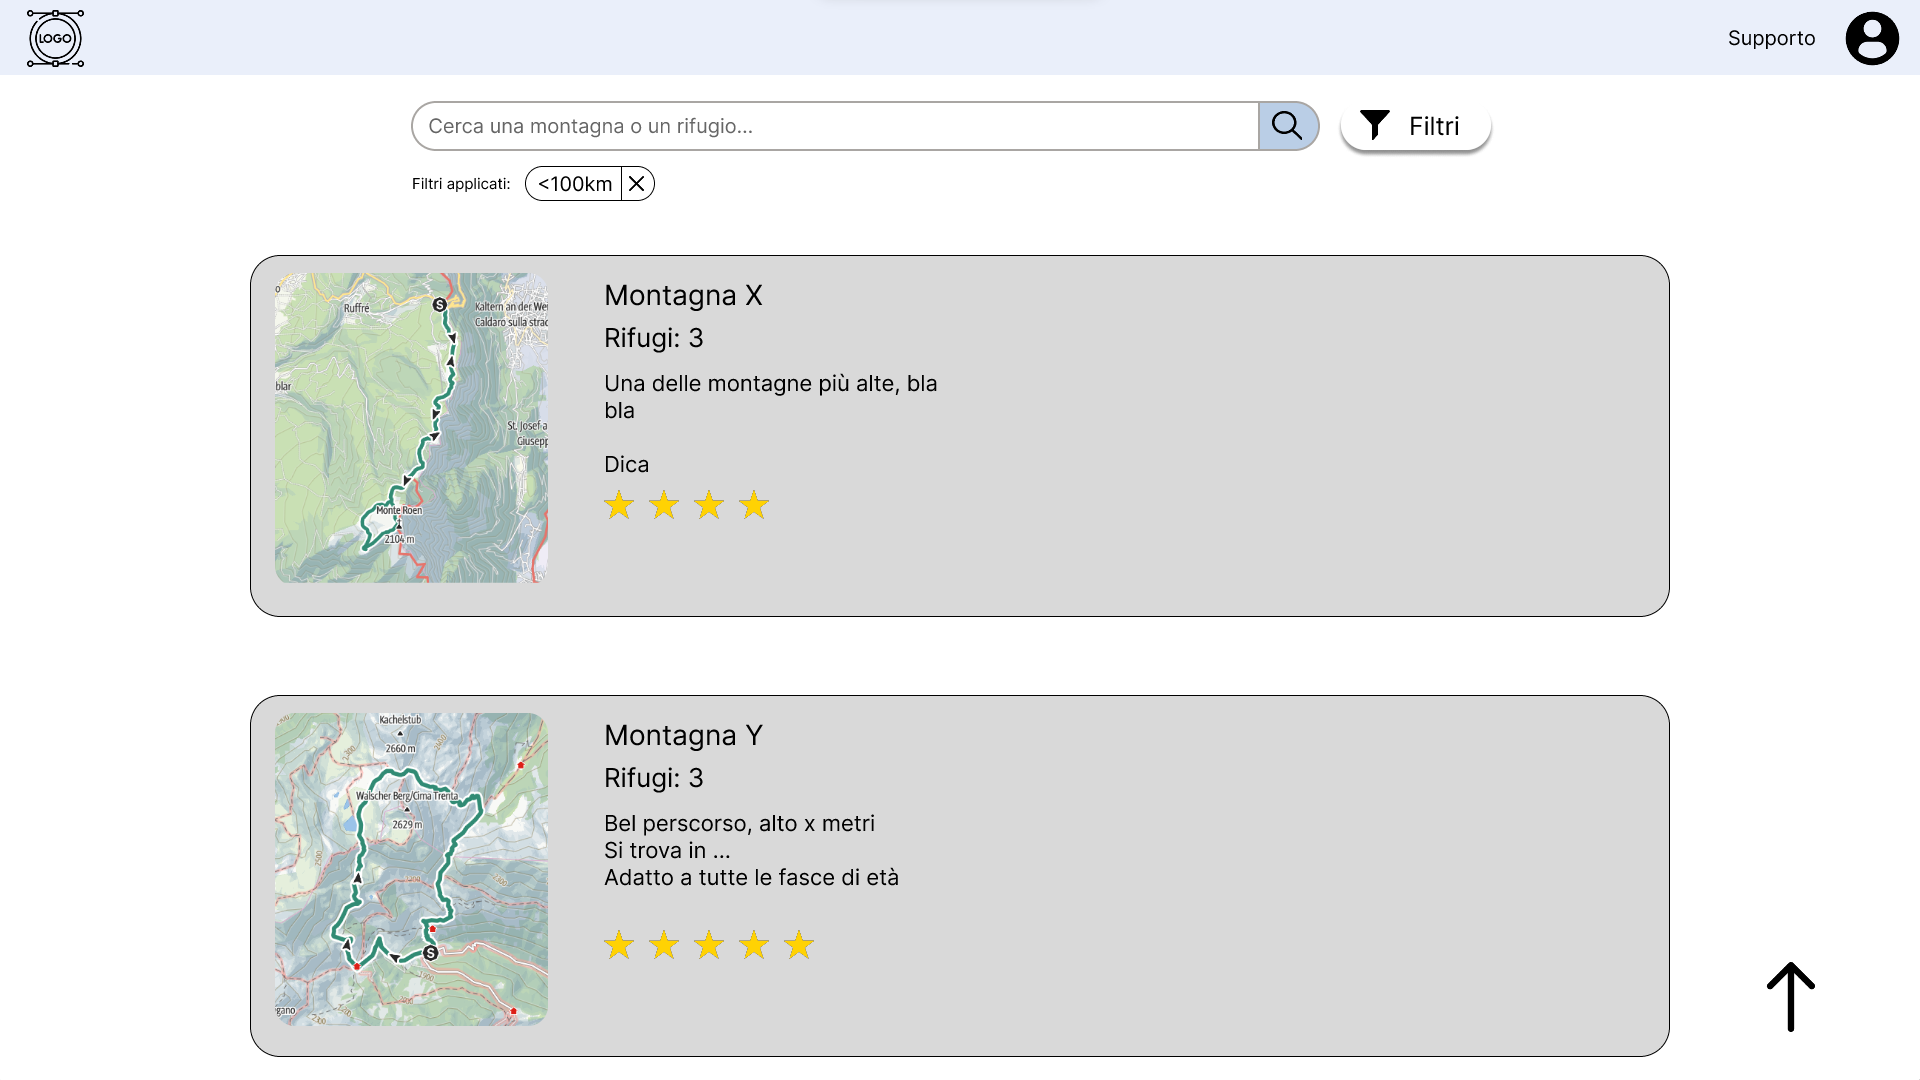
\includegraphics[width=0.6\textwidth]{img/Pagina montagne.png}
    \caption{Pagina elenco montagne (RF9)}
\end{figure}
Questa pagina darà la possibilità a qualunque tipo di utente di visionare un elenco con tutte le montagne della zona. Permetterà la ricerca di un rifugio o di una montagna tramite la barra di ricerca in alto e sarà possibile applicare dei filtri per avere risultati pertinenti a quanto si deve cercare. La freccia in basso a destrà perfetterà di tornare nella homepage.


\subsection*{FE5 Pagina account}
\begin{figure}[H]
   \centering
    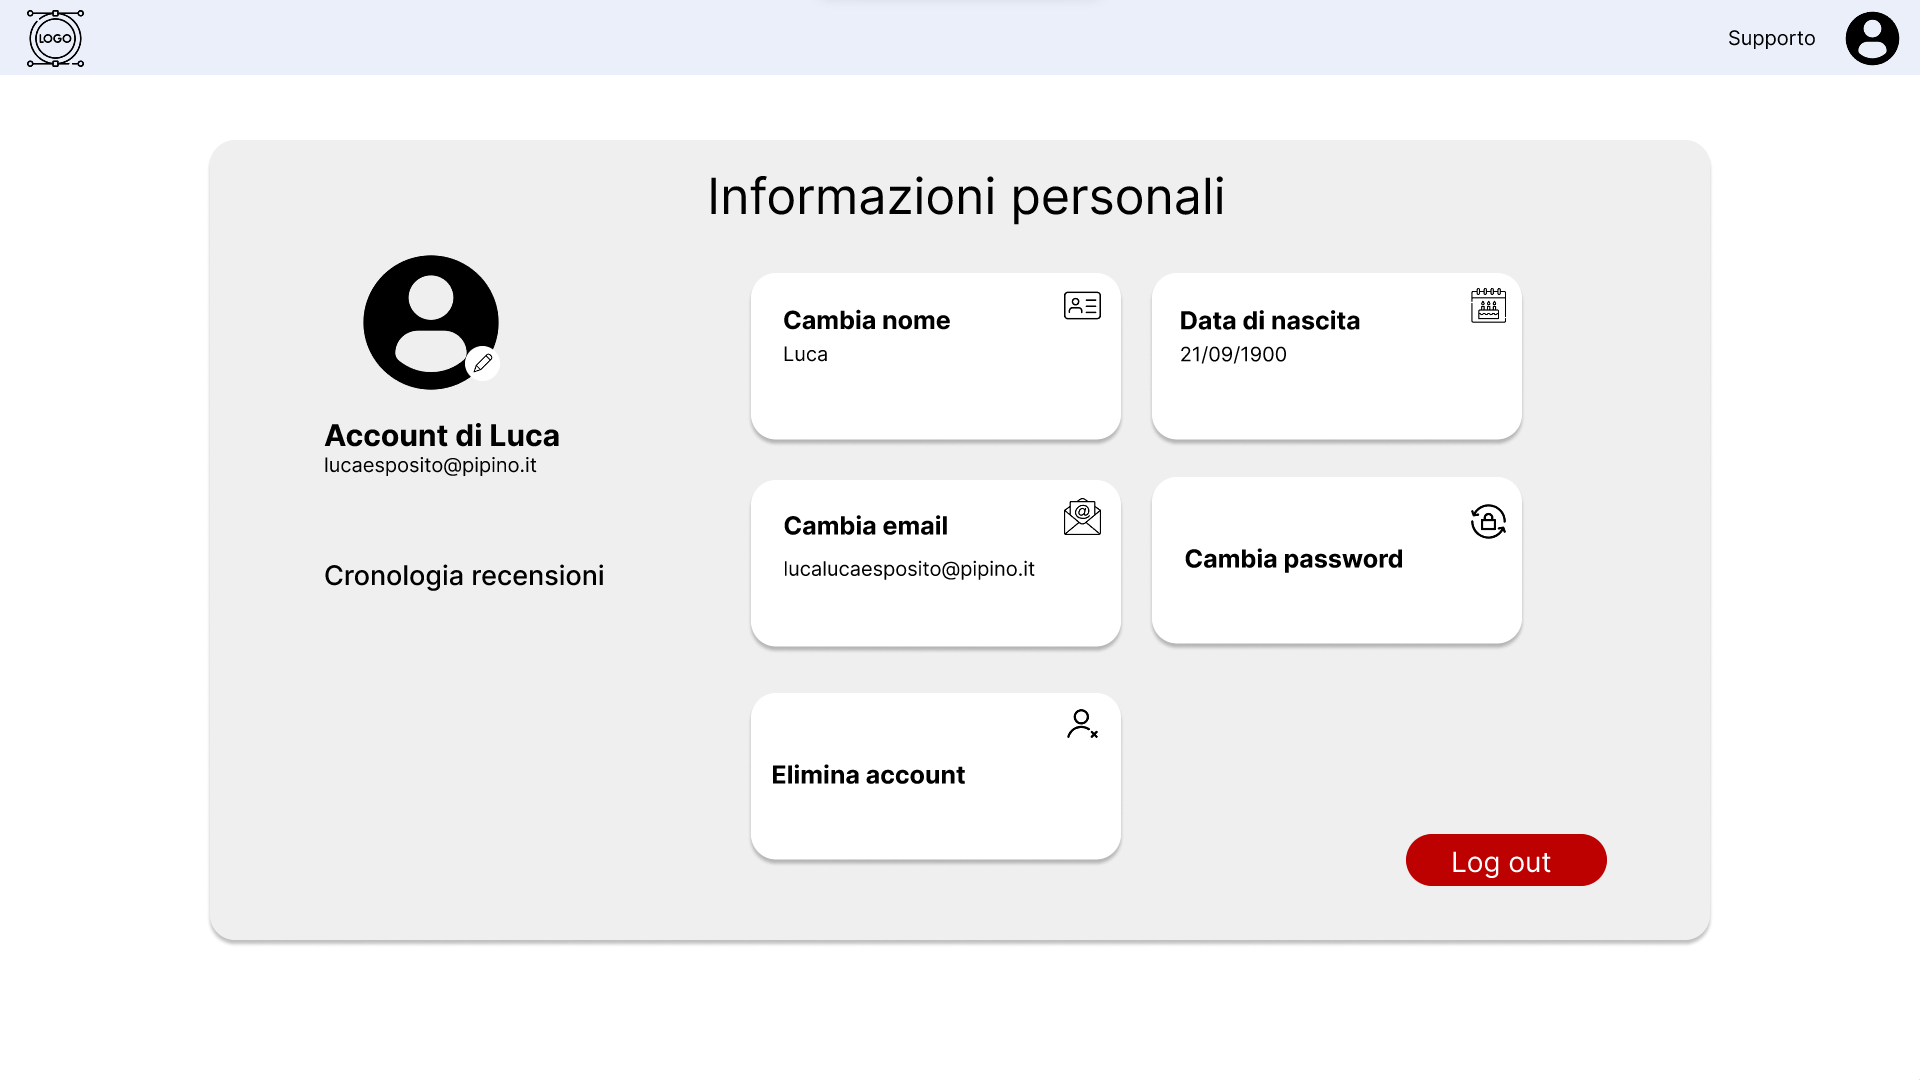
\includegraphics[width=0.6\textwidth]{img/Pagina account.png}
    \caption{Pagina account personale (RF6)}
\end{figure}

\newpage
Questa pagina permetterà all'utente di:
\begin{itemize}
    \item cambiare le informazioni personali (RF6);
    \item cambiare la password (RF6.4);
    \item richiedere l'eliminazione dell'account (RF6.5);
    \item visualizzare le recensioni effettuate con il proprio account(RF9);
\end{itemize}

\subsection*{FE5 Pagina rifugio (RF9)}
\begin{figure}[H]
   \centering
    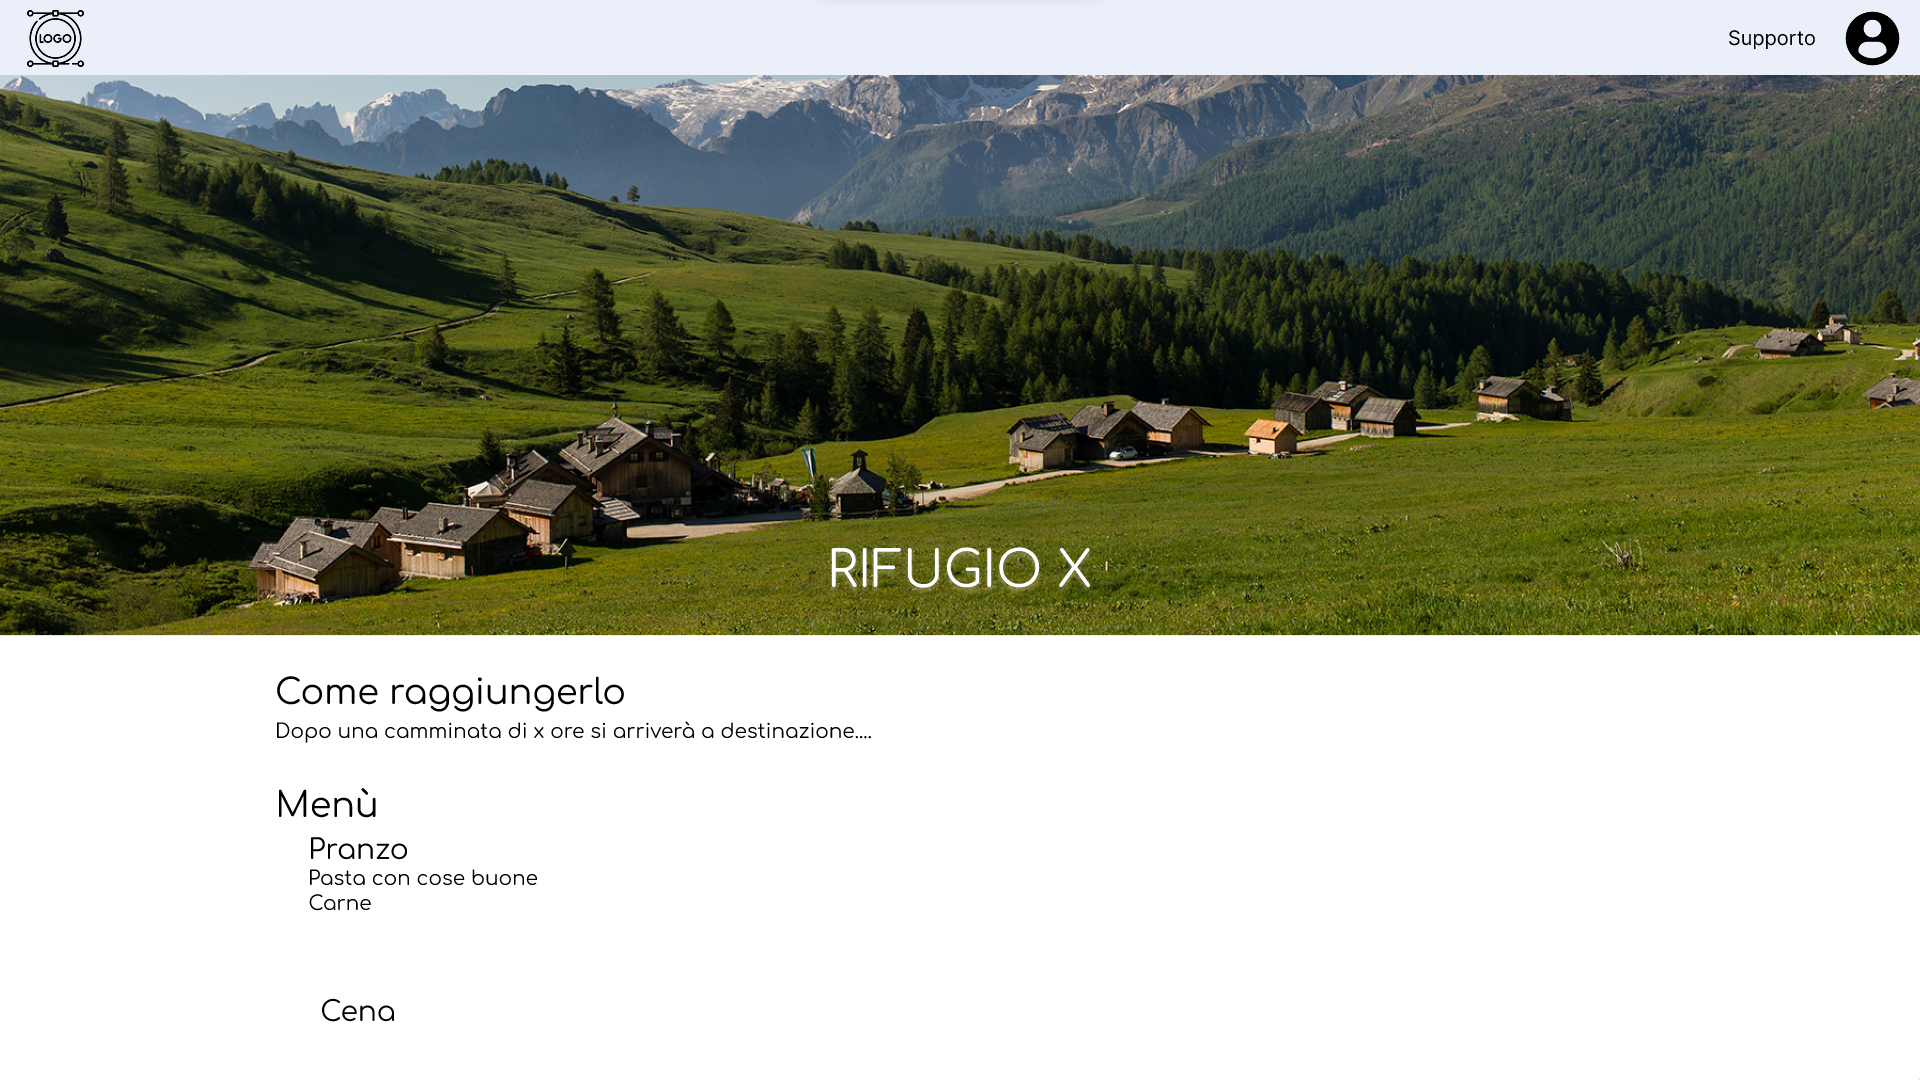
\includegraphics[width=0.6\textwidth]{img/Pagina rifugio.png}
    \caption{Pagina rifugio}
\end{figure}
Questa pagina permetterà di visualizzare un rifugio e le sue informazioni (RF9), scrollando la pagina verso il basso si troverà una sezione in cui effettuare le recensioni (RF7) e visualizzare le recensioni effettuate da altri utenti registrati.


\newpage
\section{Back-end}

Descriviamo il sito dal punto di vista dei servizi con i quale interagisce.

\subsection*{BE1 Gestore Email}
Il sito si appoggierà ad un sistema che permetterà di inviare un'email e verificare un utente che si deve registrare. Nell'email sarà presente un link per attivazione dell'account. L'utente dovrà quindi cliccare il link e loggarsi per iniziare ad utilizzare il sito.


\subsection*{BE2 Google Login API}
Il sito permetterà di registrarsi e loggarsi tramite un servizio esterno. Al momeno della registrazioni (RF1) o del login(RF2), sarà presente un pulsante per entrare utilizzando il proprio account google. Cliccato il pulsante l'utente verrà reindirizzato alla pagina di google dovre potrà inserire le proprie credenziali.

\subsection*{BE3 Google Maps API}
La web app si appoggierà alle API di Google Maps per mostrare i rifugi inseriti degli utenti(RF10). Sarà presente una mappa interattiva che mostrerà l'area circostante al rifugio.


\subsection*{BE4 Google Weather API}
Il sito sfrutterà le API di Google Weather per permettere la visualizzazione del meteo di una montagna (RF13). Questa integrazione consentirà agli utenti di accedere in modo agevole e affidabile alle informazioni meteorologiche dettagliate relative a ciascuna montagna, garantendo una previsione precisa delle condizioni meteorologiche future.
\begin{figure}[H]
   \centering
    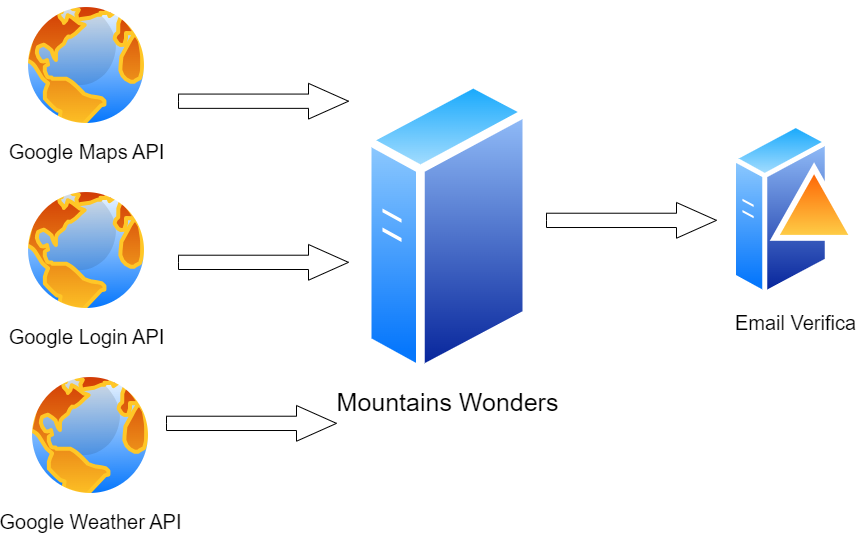
\includegraphics[width=0.5\textwidth]{img/Backend-diagram.png}
    \caption{Diagramma back-end}
\end{figure}


\end{document}